\section{The Plug-In}
Introduction to the chapter.
	What elements are there in this chapter?		
		EasyInsert
			plug-in specific elements for RWS and how they are used.
		Dialogs
		Settings		
		Device tab
		Geo tab
		Delete tab


\subsection{Dialog Windows}
Something about what dialogs does, and why we use em.

The dialogs of EasyInsert has been implemented in it's own class dialog.hpp, i.e. a subclass of QDialog, see figure~\ref{fig:subClassQWidget} for an example of a Qt subclass. This was done to keep it independent and self-contained from the rest of the plug-in. 

The constructor for the dialog class is very simple, see figure~\ref{fig:dialogConstructor}. A constructor with no WorkCell parameter is also available and passing a parent is optional, though a name must always be given to the constructor. 

\begin{figure}[h]
\centering
\lstset{language=C++} 
\begin{lstlisting}[frame=single]  
dialog::dialog(rw::models::WorkCell::Ptr wc, QString dialog, QWidget *parent)
    : QDialog(parent)
{
    _workCell = wc;
    mainLayout = new QVBoxLayout();
    setWindowTitle(dialog);
}			 
\end{lstlisting}
\caption{The dialog class constructor. A WorkCell pointer to a RW instance is passed along as a parameter. The QString parameter is the name of the dialog box and the QWidget is a pointer to the parent widget }
\label{fig:dialogConstructor} 	
\end{figure}

The dialog class is fairly simple to use and extend. A dialog is made of blocks in a vertical layout of QWidget's, i.e. a dialog instance is a composite widget containing composite widgets. Figure~\ref{fig:dialogclassblocks} shows a dialog window with four blocks initialised. All the blocks used to create all the dialog windows in the plug-in are shown in figure~\ref{fig:dialogBlocks}. These blocks are just member functions of the dialog class which returns a composite widget. So to create a dialog window as shown on figure~\ref{fig:dialogclassblocks}, a dialog instance should be constructed (in this case with a WorkCell pointer) and then simply adding the blocks to the dialog with the utility member function addToDialog(). See figure~\ref{fig:dialogWindowCode} which shows a code example on how to use the dialog class to make the dialog window as shown on figure~\ref{fig:dialogclassblocks}. 

\begin{figure}[h]
\centering
\lstset{language=C++} 
\begin{lstlisting}[frame=single]  
QString st = "Fixed Frame"; //Name of the dialog window
rw::models::WorkCell::Ptr wc = getRobWorkStudio()->getWorkCell(); //WorkCell
dialog* geoDialog = new dialog(wc,st,this); //Create the dialog window
geoDialog->addToDialog(geoDialog->createNameBox()); //Adding something
geoDialog->addToDialog(geoDialog->createFrameSelection());
geoDialog->addToDialog(geoDialog->createConfigurationBox());
geoDialog->addToDialog(geoDialog->createButtonBox());	
geoDialog->exec(); //execute/open dialog window	 
\end{lstlisting}
\caption{A sample code to illustrate how to construct the dialog window from figure~\ref{fig:dialogclassblocks}.}
\label{fig:dialogWindowCode} 	
\end{figure}

exec(), seen on figure~\ref{fig:dialogWindowCode} line 8, is an inherited public slot that executes/shows the dialog window. The dialog shown is in modal mode, meaning the window denies all user actions on any other widgets in the application. The function returns a DialogCode containing the information about whether the dialog window was accepted or rejected. The accepted or rejected information is determined by the user input to the createButtonBox() function block, since the OK button emits a accepted() signal to the accept() slot of the dialog object when pressed. Likewise the Cancel emits a rejected() signal to the reject() slot of the dialog object, though a rejected() signal is also emitted when the user presses ESC on the keyboard or the x(close) button of the dialog window.

So when a dialog window has been created and used by a user, then some functionality should be executed based on the inputs given to the dialog. That means when the function exec() returns, we need to know whether the user accepted or rejected the dialog window (pressed OK or Cancel). This is done with the inherited public function result(). The function result() returns QDialog::Accepted when the dialog was accepted and QDialog::Rejected when it was rejected (QDialog::Accepted and QDialog::Rejected are both just normal enumerators, i.e. 1 and 0). 

\begin{figure}[h]
\centering
\lstset{language=C++} 
\begin{lstlisting}[frame=single]  
geoDialog->exec();
if(geoDialog->result() == QDialog::Accepted) //Check the result
{
	std::string name = geoDialog->getNameBox(); //Get the name input
	std::string frame = geoDialog->getFrameSelection(); //Get frame selc
											 
		/*	Do something with the information    */ 
		
}
delete geoDialog; //Delete the dialog object when done using it
\end{lstlisting}
\caption{A sample code illustrating what to do after the exec()function returns.}
\label{fig:dialogAcceptedRejectedCode} 	
\end{figure}

As seen on figure~\ref{fig:dialogAcceptedRejectedCode}, after the exec() function returns, we simply check whether the result was QDialog::Accepted or not. If the result is accepted, then something should be done with the inputs given to the dialog window. We access these input via self explanatory public get-functions, e.g. the NameBox contains the name input (as seen on figure~\ref{fig:dialogAcceptedRejectedCode} line 4). After we have collected all the information we wanted out of the dialog window, then we can proceed to do something with the information, like the insertion of a frame. 


Since the dialog class is a subclass of QDialog, the position of the dialog window (opposed to a normal QDialog object) is always centred to the main application (RWS), even though a parent is passed as a parameter.

\begin{figure}[h]
	\centering
	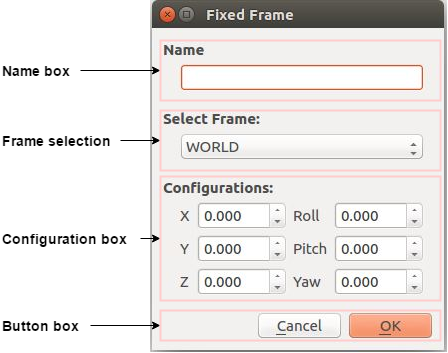
\includegraphics[scale=0.55]{Figures/dialogclassblocks.png}
	\caption{This figure shows a dialog window of adding a fixed frame to a WorkCell containing various widgets relevant to the action. }
	\label{fig:dialogclassblocks}
\end{figure}

\begin{figure}[h]
\centering
\begin{center}
  \begin{tabular}{ | l | p{7cm} |}
    \hline
    \textbf{Function blocks} 	   &   \textbf{Description}  \\ \hline
    createButtonBox()			   &   The Cancel and OK buttons. This block is used in all the dialog windows.   		\\ \hline
    createNameBox() 			   &   A line edit to specify a name.   		\\ \hline
    createCheckFramesBox()		   &   Two exclusive check boxes, i.e. only one of the boxes can be checked at a time.		\\ \hline
    createConfigurationBox() 	   &   The different configurations available to adjust regarding displacement and rotation of the inserted element. 		\\ \hline
	createConfigurationBoxCube()   &   A cube specific configuration option, i.e. the dimensions of the cube.  	\\ \hline	    
	createConfigurationBoxSphere() &   A sphere specific configuration option, i.e. the dimensions of the sphere. 	\\ \hline	
	createConfigurationBoxCone()   &   A cone specific configuration option, i.e. the dimensions of the cone.  	\\ \hline	
    createConfigurationBoxTube()   &   A tube specific configuration option, i.e. the dimensions of the tube.  	\\ \hline	
	createLibSettingsBox()		   &   This block is used to edit the settings of the device library.    	\\ \hline	 
	createFrameSelection()		   &   A way to select a parent frame for the inserted element. Default is the WORLD frame.		\\
    \hline
  \end{tabular}
\end{center}
\caption{This table summarizes all the different dialog function blocks used to construct the dialog windows in the plug-in.}
\label{fig:dialogBlocks} 
\end{figure}



widgets in the blocks has no parents? Why is this not a problem for memory management? setLayout() re-parents widgets!

Dialog is alive until parent is dead, therefore delete it when done.

Accessing the information entered into the dialog. An example ?






